\documentclass[12pt, a4paper]{article} 
\usepackage[italian]{babel}
\usepackage[utf8]{inputenc} 
\usepackage{amsmath} 
\usepackage{amssymb}
\usepackage{amsthm}
\usepackage{hyperref}
\usepackage{graphicx}
\usepackage{capt-of}
\graphicspath{{IMG/}}
\usepackage{epstopdf}
\usepackage{subcaption}
\usepackage{color}
\usepackage{booktabs}
\usepackage[table,xcdraw]{xcolor}

\title{\textbf{Politecnico di Milano}\\
		\medskip
		\begin{figure}[h]
			\centering
			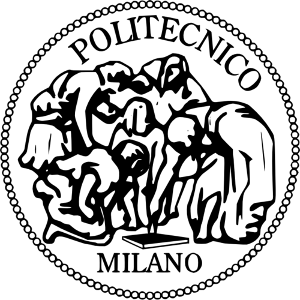
\includegraphics[scale=0.25]{logoPOLI}
		\end{figure}
		A.Y. 2015-2016\\
		\medskip 
		\medskip
		\medskip
		{\huge \textbf{DYNAMICS OF MECHANICAL SYSTEM}}\\
		\medskip 
		\medskip 
		\textit{\textbf{Motorbike Frame Analysis}}}

\author{Andrea Verzaglia - 823568}
\date{}

\begin{document}
	\maketitle
	\thispagestyle{empty}
	\clearpage
	\tableofcontents 
	\thispagestyle{empty}
	\clearpage
	\section{INTRODUZIONE}
	Il modello da studiare, che rappresenta la struttura di un telaio di una moto, è rappresentato nella figura seguente:
	\begin{figure}[h]
		\centering
		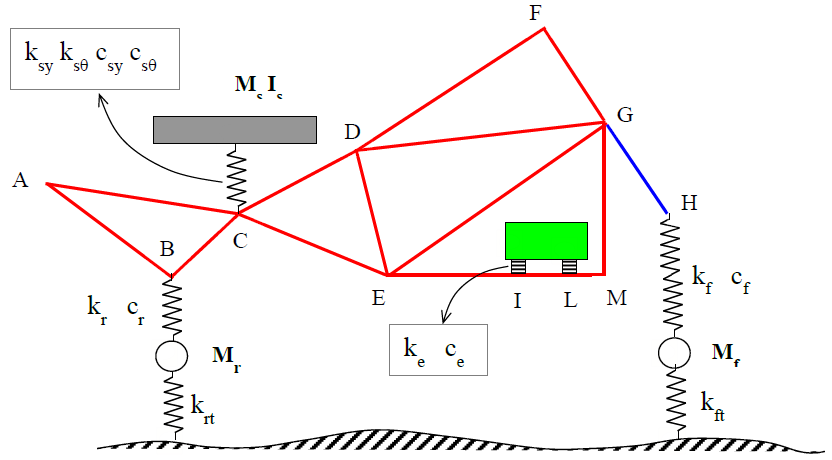
\includegraphics[scale=0.5]{frame}
		\caption{struttura telaio}
		\label{fig_1}
	\end{figure}
	
	\clearpage
	\section{RISOLUZIONE}
	\subsection{PUNTO 1}
	\textbf{DEFINIRE UN \textit{MODELLO AGLI ELEMENTI FINITI} VALIDO NEL RANGE DI FREQUENZE $0\div300Hz$}
	
	Per prima cosa è necessario definire la struttura del telaio. Si considerino i punti indicati con una lettera (vedere \textit{\underline{Figura \ref{fig_1}}}), cioè ogni punto di discontinuità, ogni punto in cui viene applicata una massa e ogni estremo di una molla come un \textit{nodo}. Per definire le posizioni degli estremi delle molle sono stati assegnati dei valori arbitrari ma coerenti alle lunghezze delle molle stesse:
	\begin{itemize}
		\item lunghezza sospensione della sella (NC): $0.150m$
		\item lunghezza sospensione del motore (IO e LP): $0.050m$
		\item lunghezza forcella (HR, sospensione ruota anteriore): $0.320m$
		\item lunghezza mono (BQ, sospensione ruota posteriore): $0.200m$
		\item lunghezza molle che modellano la rigidezza delle ruote (QS e RT): $0.100m$ 
	\end{itemize}
	Si ottiene così il seguente scenario:
	\begin{figure}[h]
		\centering
		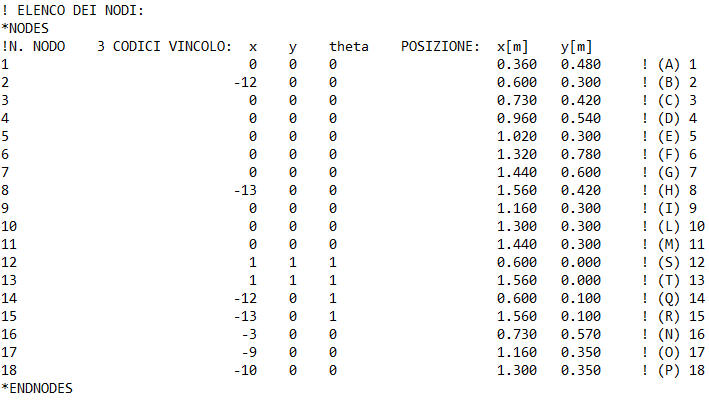
\includegraphics[scale=0.7]{Nodes}
		\caption{nodes}
	\end{figure}\\    
	\begin{figure}[h]
		\centering
		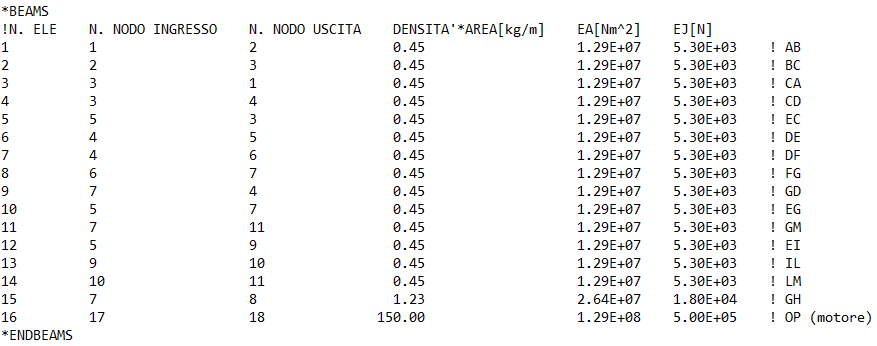
\includegraphics[scale=0.7]{Beams}
		\caption{beams}	
	\end{figure}\\
	NB: viene utilizzata la \textit{massa lineare}, ovvero la massa per metro.\\ 
	\begin{figure}[h]
		\centering
		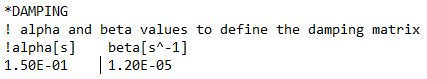
\includegraphics[scale=0.8]{Damping}
		\caption{damping (proportional damping)}
	\end{figure}\\ 
	\begin{figure}[h]
		\centering
		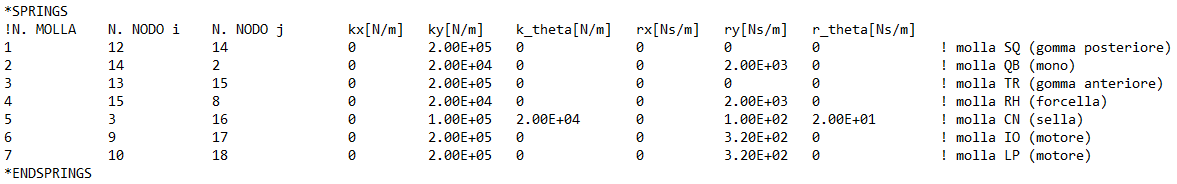
\includegraphics[scale=0.55]{Springs}
		\caption{springs}
	\end{figure}\\
	\begin{figure}[h]
		\centering
		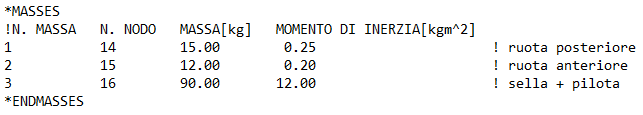
\includegraphics[scale=0.8]{Masses}
		\caption{masses}
	\end{figure}\\\\\\\\\\\\
	Infine si è verificato se il modello agli elementi finiti della struttura del telaio appena definito è valido nel range di frequenze $0\div300Hz$. Per fare questo, è necessario verificare che la \textit{prima frequenza naturale} (che è la più bassa) di ogni elemento (\textit{beam}) sia superiore alla \textit{massima frequenza} delle forze agenti sul sistema $f_{max}$ (circa \textit{1.5-3} volte superiore). Nel caso in esame $f_{max}$ è pari a $300Hz$ e poniamo $c=2$.\\
	La prima frequenza di risonanza viene calcolata con la formula
	\[f_{max,1}=\frac{1}{2 \pi c}(\frac{\pi}{L_{k}})^{2}\sqrt{\frac{E J_{k}}{m_{k}}}\]
	e i risultati ottenuti sono i seguenti 
	\begin{table}[h]
		\centering
		\resizebox{0.4\textwidth}{!}{
		\begin{tabular}{@{}|c|c|c|@{}}
			\toprule
			\textbf{TRAVE}                      & \textbf{LUNGHEZZA {[}m{]}} & \textbf{fmax {[}Hz{]}} \\ \midrule
			\cellcolor[HTML]{FE0000}\textbf{AB} & 0,300                      & 947                    \\ \midrule
			\cellcolor[HTML]{FE0000}\textbf{AC} & 0,375                      & 607                    \\ \midrule
			\cellcolor[HTML]{FE0000}\textbf{BC} & 0,177                      & 2723                   \\ \midrule
			\cellcolor[HTML]{FE0000}\textbf{CD} & 0,259                      & 1267                   \\ \midrule
			\cellcolor[HTML]{FE0000}\textbf{CE} & 0,314                      & 865                    \\ \midrule
			\cellcolor[HTML]{FE0000}\textbf{DE} & 0,247                      & 1393                   \\ \midrule
			\cellcolor[HTML]{FE0000}\textbf{DF} & 0,433                      & 455                    \\ \midrule
			\cellcolor[HTML]{FE0000}\textbf{DG} & 0,484                      & 364                    \\ \midrule
			\cellcolor[HTML]{FE0000}\textbf{EG} & 0,516                      & 320                    \\ \midrule
			\cellcolor[HTML]{FE0000}\textbf{EI} & 0,140                      & 4349                   \\ \midrule
			\cellcolor[HTML]{FE0000}\textbf{IL} & 0,140                      & 4349                   \\ \midrule
			\cellcolor[HTML]{FE0000}\textbf{LM} & 0,140                      & 4349                   \\ \midrule
			\cellcolor[HTML]{FE0000}\textbf{FG} & 0,216                      & 1821                   \\ \midrule
			\cellcolor[HTML]{FE0000}\textbf{GM} & 0,300                      & 947                    \\ \midrule
			\cellcolor[HTML]{3166FF}\textbf{GH} & 0,216                      & 2030                   \\ \midrule
			\cellcolor[HTML]{32CB00}\textbf{OP} & 0,140                      & 2314                   \\ \bottomrule
		\end{tabular}}
		\caption{}
		\label{tab_1}
	\end{table}
	\\\\
	\begin{table}[h]
		\centering
		\resizebox{0.4\textwidth}{!}{
		\begin{tabular}{@{}|c|c|c|c|c|@{}}
			\toprule
			\textbf{MATERIALE}                        & \textbf{m {[}kg/m{]}} & \textbf{EA {[}Nm\textasciicircum 2{]}} & \textbf{EJ {[}N{]}} & \textbf{Lmax {[}m{]}} \\ \midrule
			\cellcolor[HTML]{FE0000}\textbf{telaio}   & 0,45                  & 1,29E+07                               & 5,30E+03            & 0,533                 \\ \midrule
			\cellcolor[HTML]{3166FF}\textbf{forcella} & 1,23                  & 2,64E+07                               & 1,80E+04            & 0,563                 \\ \midrule
			\cellcolor[HTML]{32CB00}\textbf{motore}   & 150                   & 1,29E+08                               & 5,00E+05            & 0,389                 \\ \bottomrule
		\end{tabular}}
		\caption{}
	\end{table}
	\\\\
	Osservando la \textit{\underline{Tabella \ref{tab_1}}} è possibile affermare che il modello ideato è corretto e coerente, in quanto ogni elemento ha la prima frequenza di risonanza (che è la più bassa) maggiore di due volte la massima frequenza di eccitazione ($300Hz$).
	
	
	\subsection{PUNTO 2}
	\textbf{CALCOLARE LE \textit{FREQUENZE NATURALI} DEL SISTEMA E I RELATIVI \textit{MODI DI VIBRARE} NEL RANGE DI FREQUENZE $0\div300Hz$}
    
	Per calcolare le frequenze naturali del sistema e i corrispondenti modi di vibrare nel range $0\div300Hz$ è necessario caricare la struttura definita in precedenza come file \textit{.inp} nel programma \textit{$Matlab^{\circledR}$ "dmb\_fem2"}. Ci pensa il software a calcolare le frequenze naturali, che sono 39 essendo 39 i gradi di libertà. Ci limitiamo a mostrare nel seguito solo le combinazioni comprese nel range di frequenze richiesto.    
	\begin{figure}[h]
		\centering
		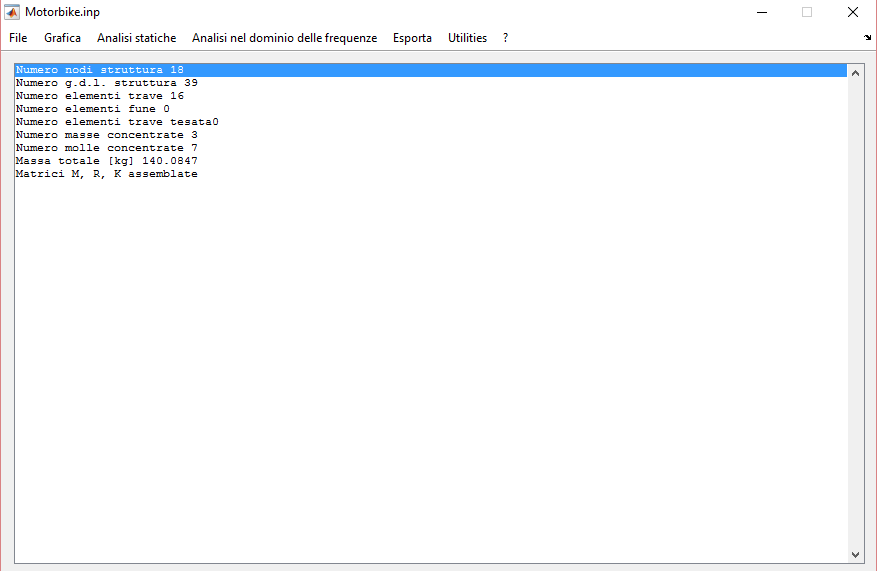
\includegraphics[scale=0.5]{GdL}
		\caption{"dmb\_fem2"}
	\end{figure}
	\begin{figure}[h]
		\centering
		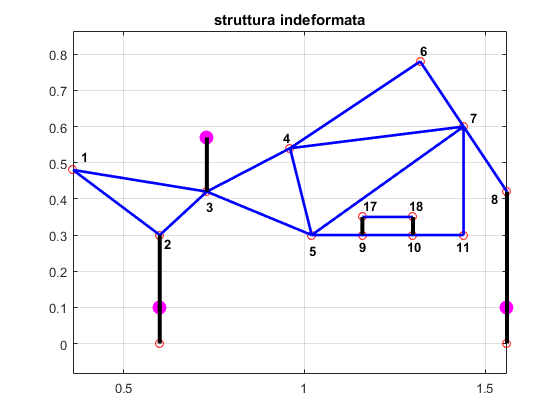
\includegraphics[scale=0.6]{struttura_indeformata}
		\caption{struttura indeformata}
	\end{figure}
	\begin{figure}[h]
		\centering
		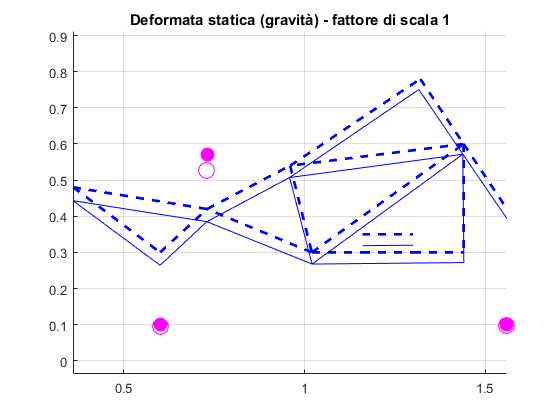
\includegraphics[scale=0.6]{deformata_statica}
		\caption{deformata statica}
	\end{figure}
	\begin{figure}[h]
		\centering
		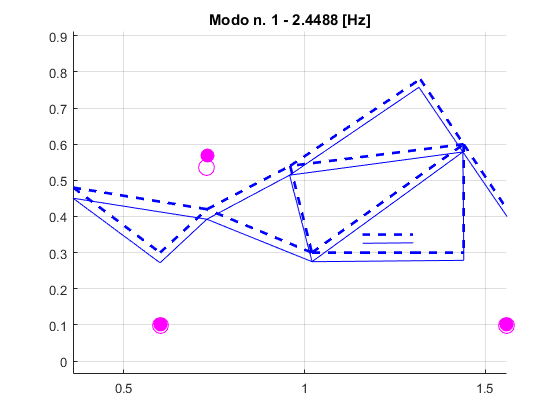
\includegraphics[scale=0.6]{modo_1}
		\caption{modo 1 (fattore di scala 0.1)}
	\end{figure}
	\begin{figure}[h]
		\centering
		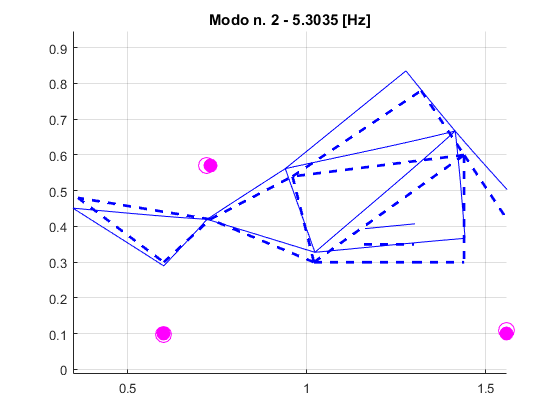
\includegraphics[scale=0.6]{modo_2}
		\caption{modo 2 (fattore di scala 0.5)}
	\end{figure}
	\begin{figure}[h]
		\centering
		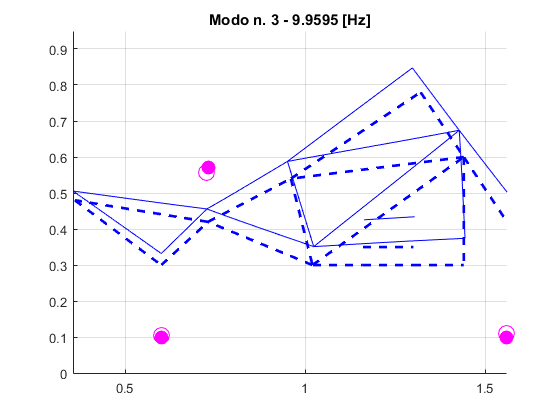
\includegraphics[scale=0.6]{modo_3}
		\caption{modo 3 (fattore di scala 0.3)}
	\end{figure}
	\begin{figure}[h]
		\centering
		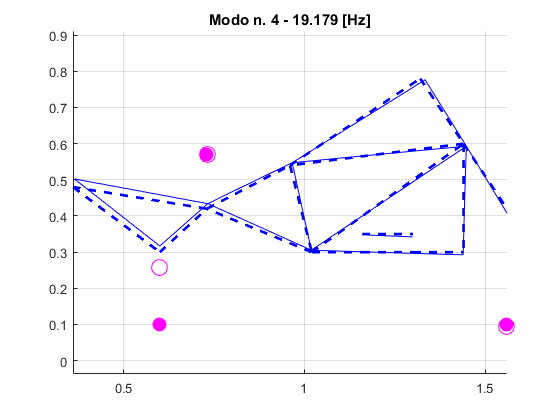
\includegraphics[scale=0.6]{modo_4}
		\caption{modo 4 (fattore di scala 0.2)}
	\end{figure}
	\begin{figure}[h]
		\centering
		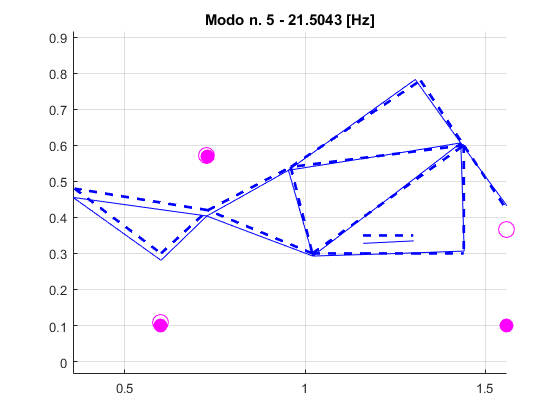
\includegraphics[scale=0.6]{modo_5}
		\caption{modo 5 (fattore di scala 0.3)}
	\end{figure}
	\begin{figure}[h]
		\centering
		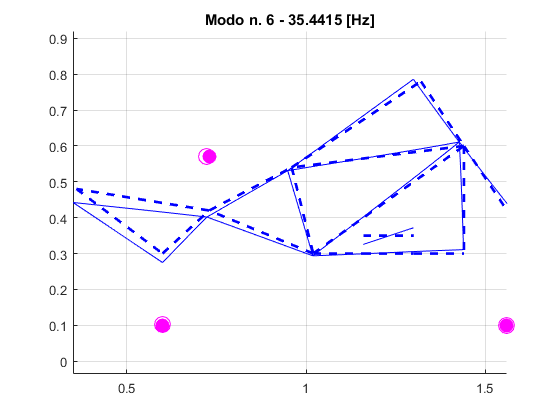
\includegraphics[scale=0.6]{modo_6}
		\caption{modo 6 (fattore di scala 0.5)}
	\end{figure}
	\begin{figure}[h]
		\centering
		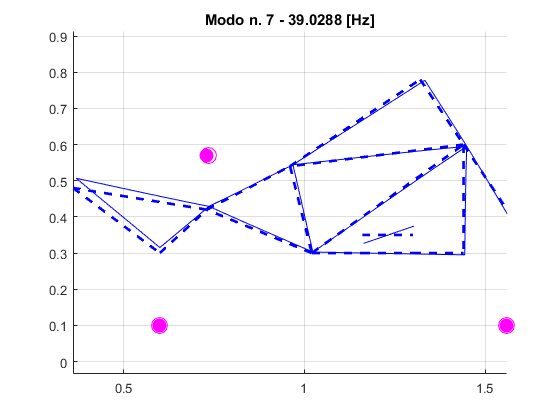
\includegraphics[scale=0.6]{modo_7}
		\caption{modo 7 (fattore di scala 0.5)}
	\end{figure}
	\begin{figure}[h]
		\centering
		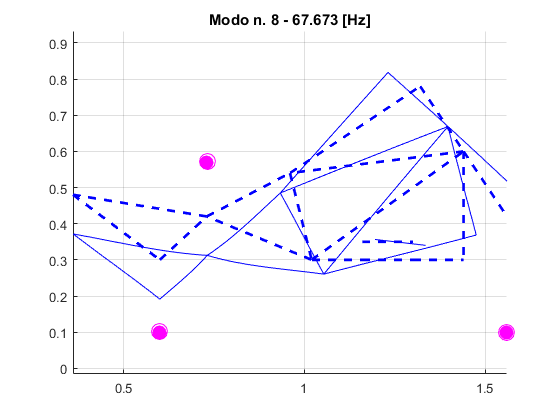
\includegraphics[scale=0.6]{modo_8}
		\caption{modo 8 (fattore di scala 0.8)}
	\end{figure}
	\begin{figure}[h]
		\centering
		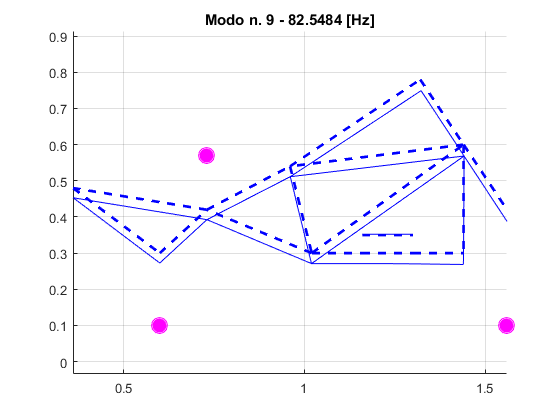
\includegraphics[scale=0.6]{modo_9}
		\caption{modo 9 (fattore di scala 0.1)}
	\end{figure}
	
	
	\clearpage
	\subsection{PUNTO 3}
	\textbf{CALCOLARE LA \textit{RISPOSTA IN FREQUENZA} (FRF) NEL RANGE DI FREQUENZE $0\div300Hz$ CON STEP $0.1Hz$:
	\begin{itemize}
			\item [a)] INPUT: forza verticale sulla sella\\ 
			OUTPUT: accelerazione verticale della sella
			\item [b)] INPUT: forza verticale sul mozzo della della ruota anteriore $M_{f}$\\
			OUTPUT: accelerazione verticale della sella	
			\item [c)] INPUT: forza verticale sul mozzo della ruota posteriore $M_{r}$\\
			OUTPUT: accelerazione verticale della sella
			\item [d)] INPUT: due forze verticali, in fase e applicate nei punti di connessione tra le sospensioni del motore e il telaio (punti I e L)\\
			OUTPUT: accelerazione verticale della sella 			 
	\end{itemize}}
	
	Anche in questo caso ci pensa il software, basta semplicemente inserire i nodi di ingresso e di uscita. Riportiamo nel seguito i \textit{diagrammi di Bode} (modulo e fase) delle risposte in frequenza.\\
	NB: i valori delle forzanti sono unitari. 
	\begin{figure}[h]
		\centering
		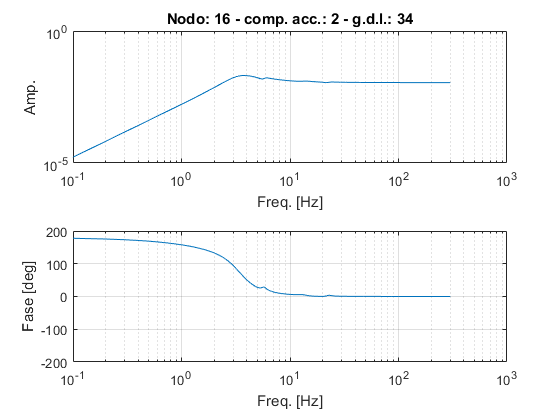
\includegraphics[scale=0.8]{FRF_1}
		\caption{FRF\_a}
	\end{figure}
	\begin{figure}[h]
		\centering
		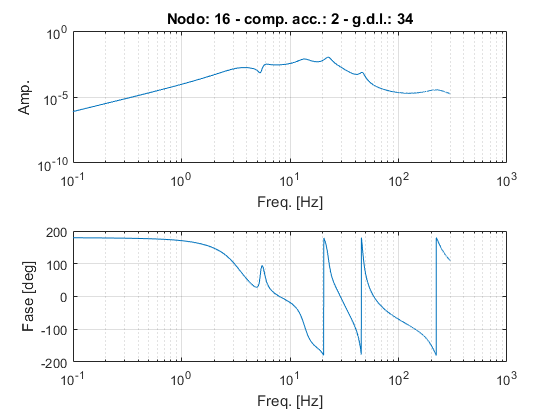
\includegraphics[scale=0.8]{FRF_2}
		\caption{FRF\_b}
	\end{figure}
	\begin{figure}[h]
		\centering
		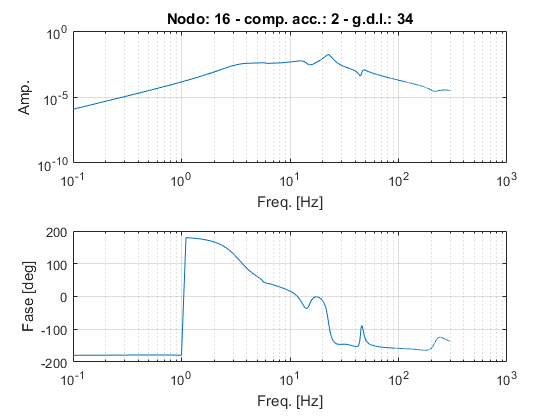
\includegraphics[scale=0.8]{FRF_3}
		\caption{FRF\_c}
	\end{figure}
	\begin{figure}[h]
		\centering
		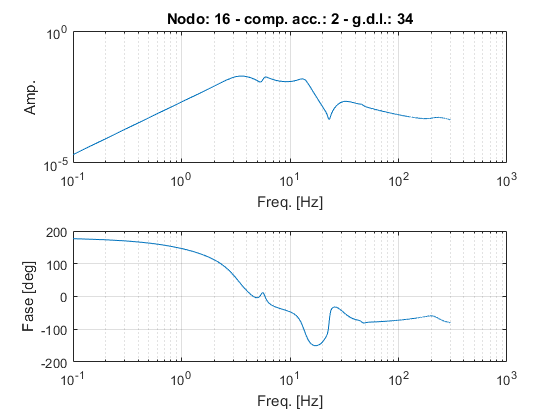
\includegraphics[scale=0.8]{FRF_4}
		\caption{FRF\_d}
	\end{figure}
	
	\clearpage
	\subsection{PUNTO 4}
	\textbf{CALCOLARE LA \textit{RISPOSTA IN FREQUENZA} (FRF) NEL RANGE DI FREQUENZE $0\div300Hz$ CON STEP $0.1Hz$:
	\begin{itemize}
		\item INPUT: i seguenti spostamenti verticali applicati alla ruota anteriore e posteriore:
		\begin{enumerate}
			\item [a)]$y_{f}=y_{r}=cos(\Omega t)$ ; $\Omega = 2 \pi f$
			\item [b)]$y_{f}=cos(\Omega t)$ ; $y_{r}=cos(\Omega t + \varphi)$ ; $\Omega = 2 \pi f$
		\end{enumerate}
		OUTPUT: accelerazione verticale della sella  
	\end{itemize}}
	In questo caso, rispetto al punto precedente, non è possibile utilizzare il software in quanto gli ingressi richiesti corrispondono a spostamenti verticali applicati alla ruota anteriore e posteriore, che sono nodi vincolati. E' necessario quindi scrivere uno \textit{script} (\textit{Motorbike.m}) \textit{$Matlab^{\circledR}$} nel quale gli spostamenti applicati ai vincoli sono stati definiti in questo modo
	\[x\_c=[0;\medspace y\_dietro;\medspace 0;\medspace 0;\medspace y\_davanti;\medspace 0;\medspace 0;\medspace 0]\] 
	guardando la \textit{IDB matrix} per capire in quale posizione del vettore inserire gli spostamenti.\\
	Le due risposte in frequenza sono le seguenti:
	\begin{figure}[h]
		\centering
		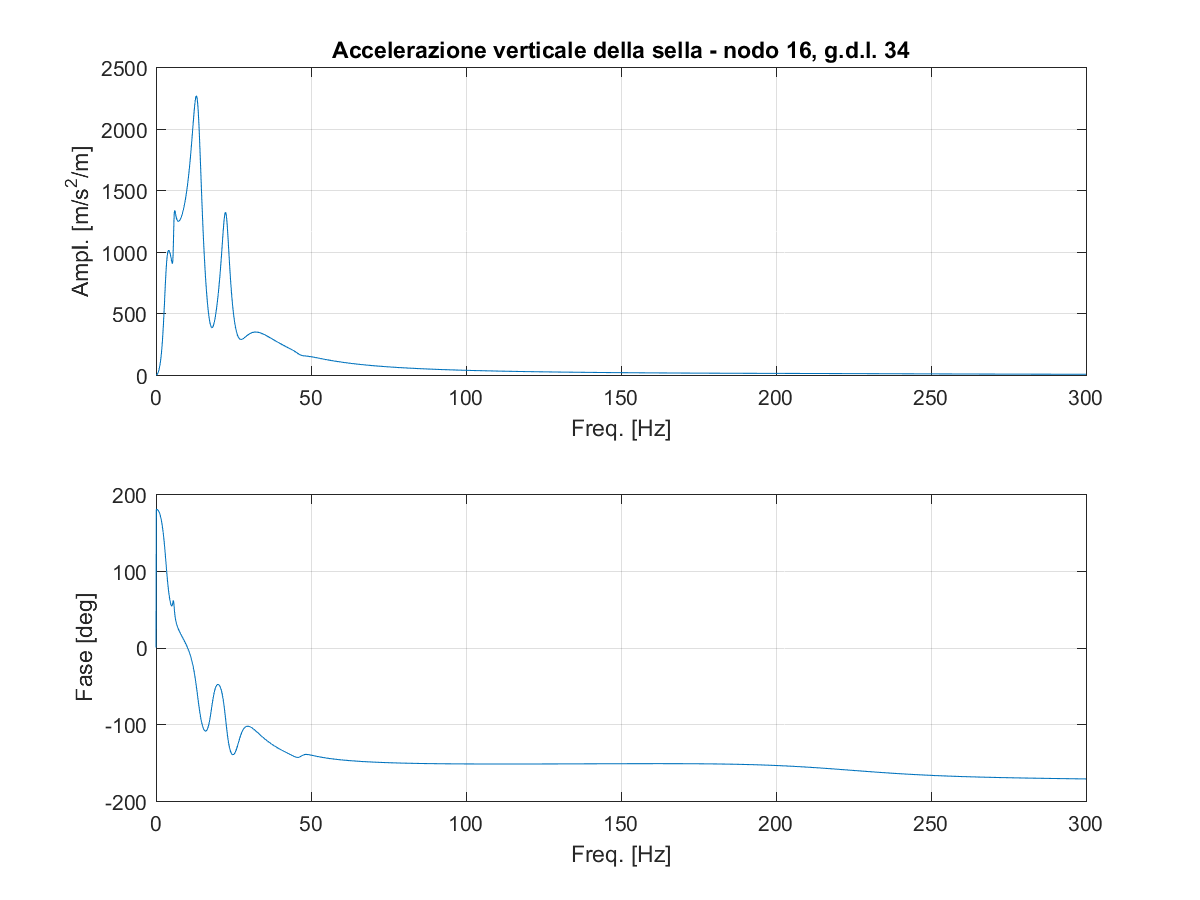
\includegraphics[scale=0.8]{FRF_5}
		\caption{FRF\_a}
	\end{figure}
	\begin{figure}[h]
		\centering
		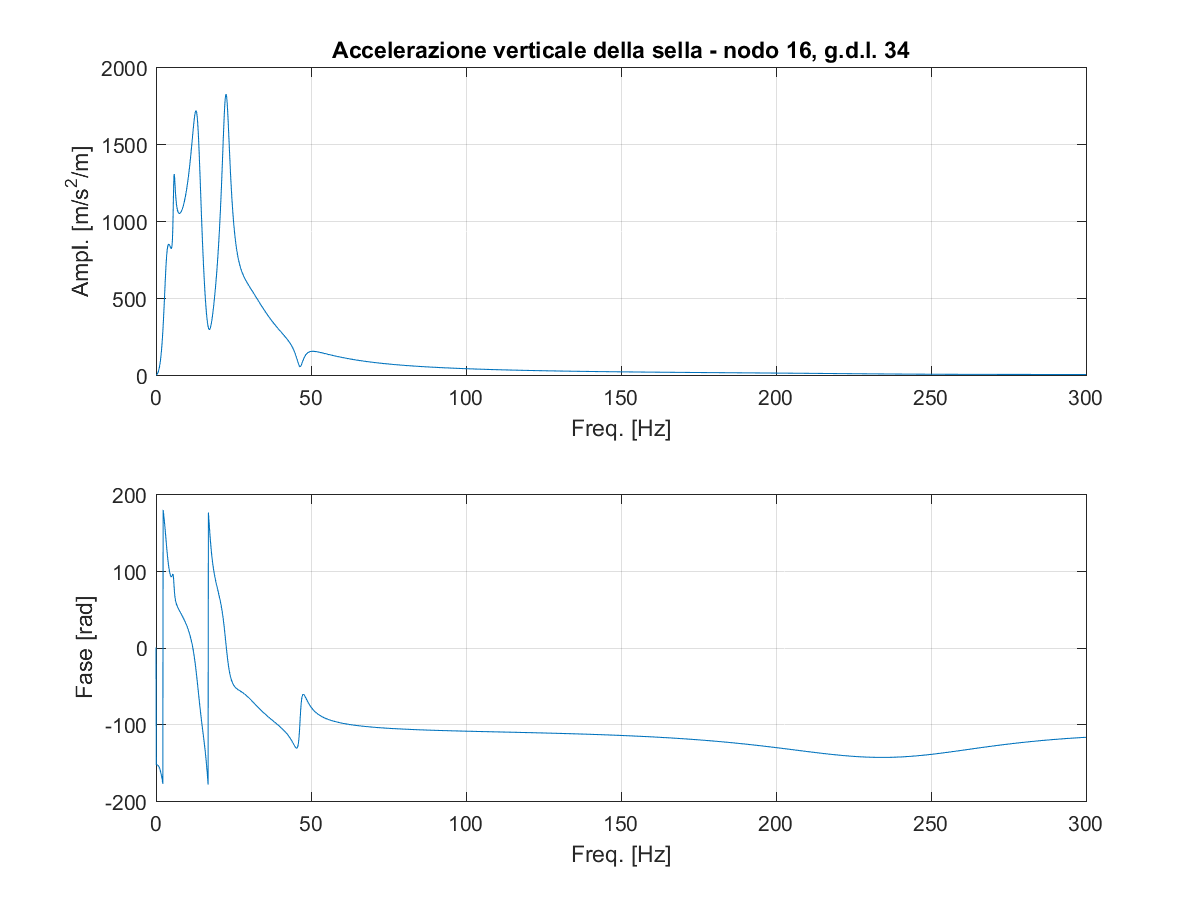
\includegraphics[scale=0.8]{FRF_5b}
		\caption{FRF\_b}
	\end{figure}
	
	\clearpage
	\subsection{PUNTO 5}
	\textbf{CALCOLARE LA RISPOSTA DEL TELAIO APPLICANDO UNO SPOSTAMENTO VERTICALE DOVUTO ALLA STRADA SCONNESSA, ASSUMENDO LA SEGUENTE FUNZIONE $y(\xi)$ PER DESCRIVERE IL PROFILO DELLA STRADA COME FUNZIONE DELLA POSIZIONE LONGITUDINALE $\xi$ DEL PUNTO DI CONTATTO:
		\[y=\sum_{i=1}^{3} A_{i} cos(\frac{2 \pi}{\lambda_{i}} \xi)\]
	RIPORTARE I SEGUENTI RISULTATI GRAFICI:
	\begin{enumerate}
		\item [a)]\textit{spettro} degli spostamenti applicati alle ruote
		\item [b)]\textit{risposta in frequenza} dello spostamento verticale della sella dovuto agli spostamenti verticali applicati ad ogni punto di contatto delle ruote
		\item [c)]\textit{spettro} dello spostamento verticale della sella
		\item [d)]\textit{storia temporale} dello spostamento verticale della sella
	\end{enumerate}
	CALCOLARE INFINE I VALORI DI \textit{V} CHE PORTANO IL TELAIO IN RISONANZA.}
	\\\\Per prima cosa è necessario ricostruire il \textit{profilo stradale} in funzione del \textit{tempo} anziché dello spazio, come somma di 3 armoniche $y_{1}$, $y_{2}$ e $y_{3}$. Conoscendo la velocità costante $V$ della moto basta semplicemente utilizzare la trasformazione $\xi=V\cdot t$\medspace:\\
	\[y_{1}=A_{1} \cdot cos(\frac{2 \pi}{\lambda_{1}} \cdot V \cdot t)\]
	\[y_{2}=A_{2} \cdot cos(\frac{2 \pi}{\lambda_{2}} \cdot V \cdot t)\]
	\[y_{3}=A_{3} \cdot cos(\frac{2 \pi}{\lambda_{3}} \cdot V \cdot t)\] 
	\[y\_davanti=y_{1}+y_{2}+y_{3}\]
	Quanto fatto finora riguarda lo spostamento della ruota anteriore; bisogna fare lo stesso anche per la ruota posteriore tenendo presente lo sfasamento di un certo intervallo temporale, calcolabile conoscendo la distanza tra la ruota anteriore e quella posteriore che è pari a $0.96m$:\\
	\[t_{0}=\frac{0.96}{V}\]
	\[y_{1}=A_{1} \cdot cos(\frac{2 \pi}{\lambda_{1}} \cdot V \cdot (t-t_{0}))\]
	\[y_{2}=A_{2} \cdot cos(\frac{2 \pi}{\lambda_{2}} \cdot V \cdot (t-t_{0}))\]
	\[y_{3}=A_{3} \cdot cos(\frac{2 \pi}{\lambda_{3}} \cdot V \cdot (t-t_{0}))\] 
	\[y\_dietro=y_{1}+y_{2}+y_{3}\]\\ 
	Sempre con l'ausilio di \textit{$Matlab^{\circledR}$} si ottengono così i seguenti spostamenti applicati alle ruote e i corrispondenti spettri:
	\\
	\begin{center}
		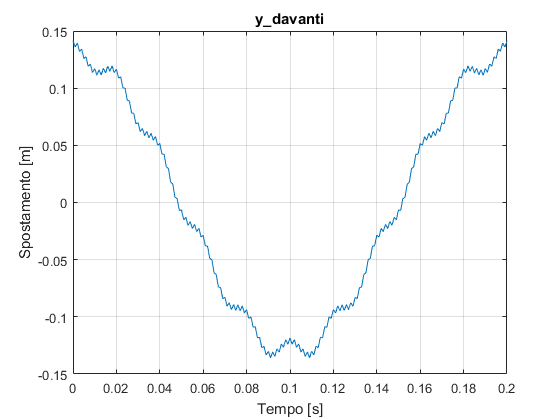
\includegraphics[scale=0.8]{y_davanti}
	\captionof{figure}{spostamento ruota anteriore}
	\end{center}

	\begin{center}
		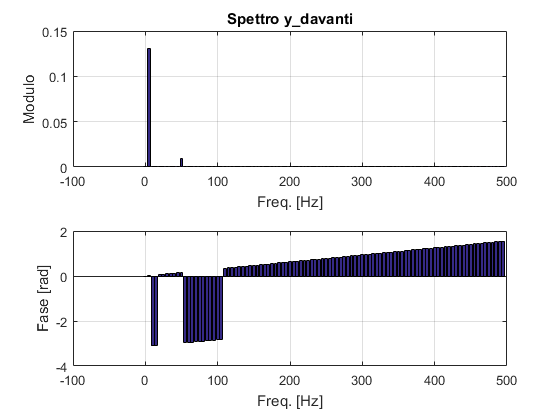
\includegraphics[scale=0.8]{spettro_y_davanti}
	\captionof{figure}{spettro spostamento ruota anteriore}
	\end{center}
	
	\begin{center}
		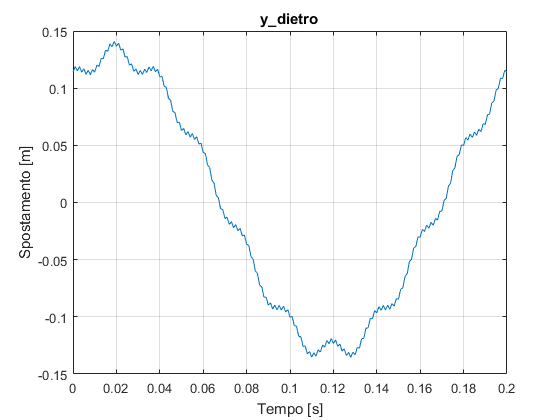
\includegraphics[scale=0.8]{y_dietro}
	\captionof{figure}{spostamento ruota posteriore}
	\end{center}
		
	\begin{center}
		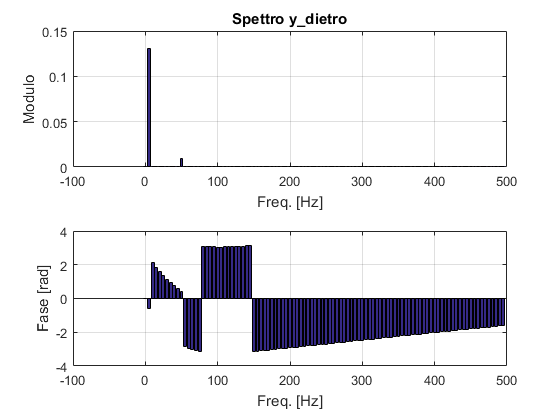
\includegraphics[scale=0.8]{spettro_y_dietro}
	\captionof{figure}{spettro spostamento ruota posteriore}
	\end{center}
	\clearpage
	Ricaviamo ora la \textit{risposta in frequenza} dello spostamento verticale della sella dovuto agli spostamenti applicati alle ruote, lo \textit{spettro} e la sua \textit{storia temporale}: 
	\\  
	\begin{center}
		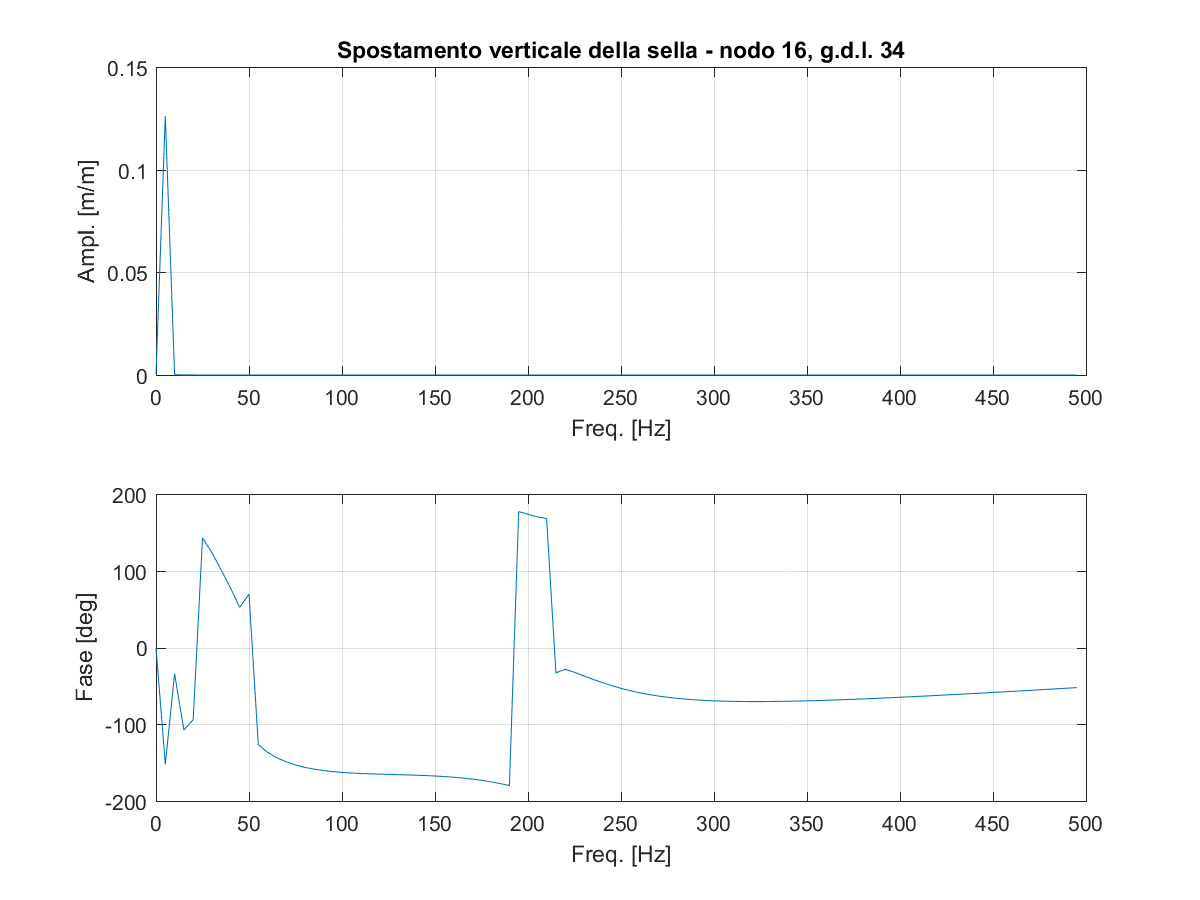
\includegraphics[scale=0.8]{FRF_6}
		\captionof{figure}{FRF}
	\end{center}
	
	\begin{center}
		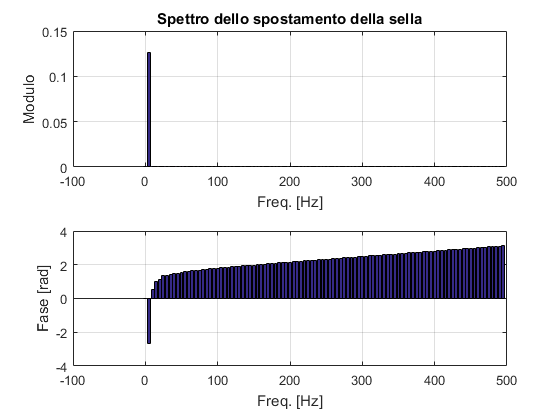
\includegraphics[scale=0.8]{spettro_5b}
		\captionof{figure}{spettro}
	\end{center}
	
	\begin{center}
		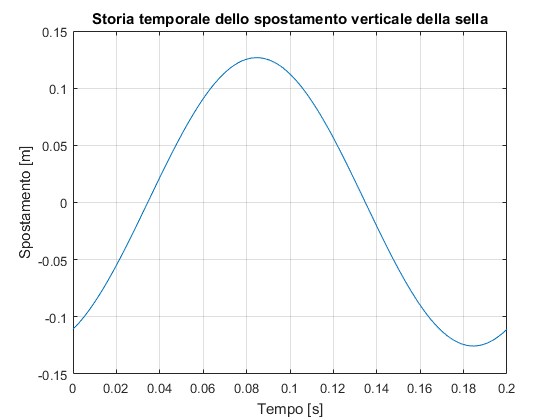
\includegraphics[scale=0.8]{storiatemporale_5b}
		\captionof{figure}{storia temporale}
	\end{center}
	\clearpage
	Come ultima domanda del punto 5 è richiesto di calcolare i valori della vlocità \textit{V} della moto che portano a una condizione di risonanza per la struttura. Ricordiamo che abbiamo una condizione di risonanza ogni qual volta che la frequenza della forzante è uguale ad una delle frequenze naturali del sistema.\\
	La \textit{frequenza di eccitazione} è data da:
	\[freq_{eccitazione}=\dfrac{V}{\lambda}\]
	Imponendo che:
	\[freq_{eccitazione}=freq_{naturale}\]
	Le velocità che portano ad una condizione di risonanza sono date da:
	\[V=freq_{naturale} \cdot \lambda\]
	Come esempio, si consideri la risonanza della sella ($f_{n}=35.4415Hz$)
	\[\lambda_{1} \Rightarrow V_{1}= 354.4 \frac{m}{s}\]
	\[\lambda_{2} \Rightarrow V_{2}= 35.4 \frac{m}{s}\]
	\[\lambda_{3} \Rightarrow V_{3}= 3.5 \frac{m}{s}\]
	
	\clearpage
	\subsection{PUNTO 6}
	\textbf{MODIFICARE LE \textit{SOSPENSIONI DEL MOTORE} CAMBIANDO LA \textit{RIGIDEZZA} $k_{e}$ E IL \textit{COEFFICIENTE DI SMORZAMENTO} $c_{e}$ IN MODO DA RIDURRE LE VIBRAZIONI DEL TELAIO, ASSUMENDO:
	\begin{itemize}
		\item velocità angolare del motore pari a $1000rpm$
		\item massima deflessione statica delle sospensioni del motore pari a $1mm$ 
	\end{itemize}}
	Un qualsiasi sistema reale è nella maggior parte dei casi un sistema vincolato ad un telaio, cioè è vincolato all'ambiente circostante esterno. Se questo sistema è soggetto a vibrazioni, quest'ultime saranno trasmesse attraverso i vincoli all'ambiente circostante, causando disturbi. Premesso che è ovviamente impossibile pensare di poter eliminare del tutto tale circostanza, il problema dell'\textit{isolamento delle vibrazioni} indotte da un sistema vibrante deve essere visto come il tentativo di ridurre il più possibile l'intensità delle forze trasmesse dal sistema al basamento. Con questo fine è necessario intervenire sui valori dei parametri che caratterizzano il \textit{sistema ammortizzante} o \textit{antivibrante}, costituito da molle e smorzatori di tipo viscoso.\\
	In ambito tecnico, la \textit{bontà} del risultato dell'isolamento può essere valutata attraverso il valore assunto da un parametro specifico detto \textit{coefficiente di trasmissibilità T}, definito come il rapporto fra il valore massimo della forza trasmessa al basamento ed il valore massimo della forza eccitatrice esterna.
	\[T=\frac{(F_{T})max}{F_{0}}\]
	Tale grandezza rapporta quindi l'ampiezza della forza trasmessa dall'antivibrante al basamento ($F_{T}$) con l'ampiezza della forza che sarebbe trasmessa alla fondazione senza l'interposizione dell'antivibrante ($F_{0}$).       
	\begin{center}
		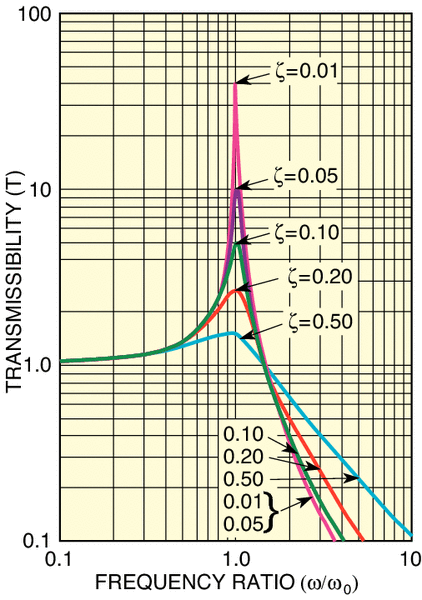
\includegraphics[scale=0.8]{trasmissione}
		\captionof{figure}{diagramma della trasmissibilità T}
	\end{center}
	In termini di frequenze, considerando i valori che assume la trasmissibilità, si può notare che per frequenze molto basse, alla struttura di sostegno viene trasmessa una forza di intensità pari a quella che agisce sulla macchina. All'aumentare della frequenza della forza eccitante aumenta la forza trasmessa al basamento, che diventa infinitamente grande in condizione di risonanza. Per frequenze superiori alla frequenza naturale la forza trasmessa decresce rapidamente raggiungendo il valore della forza impressa in corrispondenza della frequenza $\frac{f}{f_{n}}=\sqrt{2}$, per poi decrescere ancora all'aumentare della frequenza forzante o eccitante. Quest'ultima zona è quella considerata \textit{utile}: in altre parole, tenendo presente quanto visto circa il fattore \textit{T}, è possibile affermare che il principio base dell'isolamento consiste nello scegliere un elemento visco-elastico tale per cui la frequenza propria del sistema macchina-elemento antivibrante ($f_{n}$) risulti inferiore alla più bassa frequenza componente lo spettro della macchina ($f$). Quindi, in definitiva, l'obiettivo è porre la frequenza di risonanza del sistema in esame al di sotto della più bassa frequenza di eccitazione del sistema.   
	\[\omega_{motore}=\frac{1000 \cdot 2 \cdot \pi}{60}\]
	\[f_{motore}=\frac{\omega_{motore}}{2 \cdot \pi}\]   
	Così facendo la frequenza di eccitazione sul motore risulta $16.67Hz$.\\
	La consegna fornisce un limite sulla \textit{deflessione statica massima} delle sospensioni del motore pari a $1mm$. Ciò significa che il peso del motore, diviso su entrambe le sospensioni, deve portare ad una deflessione statica massimo di $1mm$, per cui:
	\[\frac{m_{motore}}{2} \cdot g = k_{e} \cdot x \] 
	Sapendo che la massa del motore è pari a $21kg$, si ottiene che:
	\[k_{e}(minimo)=\frac{m_{motore} \cdot g}{2 \cdot x_{massimo}}= 102900\frac{N}{m}\]  
	Per la tecnica dell'isolamento delle vibrazioni è necessario minimizzare il coefficiente di trasmissibilità, rendendo $\frac{f}{f_{n}}$ maggiore di $\sqrt{2}$ (più grande è, meglio è). Dobbiamo quindi rendere la frequenza naturale la più piccola possibile rispetto alla frequenza di eccitazione ($16.67Hz$), tenendo in considerazione la richiesta della deflessione massima che impone $k_{e}(minimo) = 102900\frac{N}{m}$, per cui:
	\[\omega = \sqrt{\frac{k}{m}} = 2 \cdot \pi \cdot f \]
	\[f_{n}= \frac{\sqrt{\frac{2 \cdot k_{e}}{m_{motore}}}}{2 \cdot \pi} \]
	Tuttavia, la frequenza naturale minima ottenibile risulta $15.76Hz$ che porta ad un rapporto $\frac{f}{f_{n}}=1.05$ che è ben al di sotto della soglia $\sqrt{2}$ presa come obiettivo. Anzi, ponendo la frequenza naturale pari a quel valore si ha una forza trasmessa al telaio maggiore del caso senza sospensioni. Per risolvere questo problema si può pensare di mantenere la rigidezza della molla uguale, ma prendere il coefficiente di smorzamento pari al \textit{valore critico}, in modo da rendere il più basso possibile il picco del coefficiente di trasmissibilità. Tale picco, infatti, verrà attraversato sicuramente essendo il motore a $1000\frac{giri}{min}$ e quindi la velocità angolare del motore non potrà che aumentare.
	\[c = 2 \cdot m_{motore} \cdot \omega_{n} = 5.8 \cdot 10^{3} \frac{Ns}{m} \]  
	   
	
\end{document}